% ----------------------------------------------------------
\chapter{Modelo Aeroservoelástico}\label{cap:modelo}
% ----------------------------------------------------------
A modelagem matemática do sistema aeroservoelástico deve ser realizada de forma a descrever a interação das forças inercias, deformações estruturais e carregamentos aerodinâmicos. Grande parte dos problemas aeroelásticos são abordados a partir de uma metodologia que utiliza uma descrição no domínio da frequência para os fenômenos dinâmicos, o que representa uma vantagem já que modelagens clássicas para determinação dos esforços aerodinâmicos apresentam os resultados em função da frequência reduzida \cite{book:Wright-Cooper}. Entretanto, essa descrição considera somente movimentos totalmente desenvolvidos, isto é, representados por sinais harmônicos e, apesar de apresentar grande representatividade de modelagem de movimentos oscilatórios, o estudo do comportamento transitório não é possível a partir desta metodologia \cite{book:Fung}.

Com o objetivo de considerar o comportamento transitório causado por condições iniciais não-nulas, entradas forçadas e perturbações, uma abordagem no domínio do tempo é necessária. Para isso, os esforços aerodinâmicos, cuja dependência da frequência representa os efeitos não estacionários, devem ser tratados de forma que tal dependência possa ser representada no domínio do tempo \cite{book:Wright-Cooper}. A modelagem no tempo pode ser feita utilizando uma representação no espaço de estados, o que representa vantagens na aplicação do modelo em projeto de leis de controle, sobretudo na realimentação de estados, que é a técnica a ser adotada no presente trabalho.

Neste capítulo será feita a modelagem do sistema de estudo, composto de uma seção transversal bidimensional de asa com \textit{flap} no bordo de fuga atuando como superfície de controle, vide Figura \ref{fig:cap2:sistema-fisico}. Em particular, serão desenvolvidas as equações do movimento que descrevem o sistema e, posteriormente, os esforços generalizados (carregamentos aerodinâmicos) são tratados utilizando uma metodologia designada \glsxtrfull{RFA}, baseada em \textcite{art:RogerRFA1977}. Por fim, as equações do movimento e a aproximação dos termos aerodinâmicos são integradas, obtendo o modelo completo no espaço de estados.

% ----------------------------------------------------------

% ----------------------------------------------------------
\section{Descrição do Sistema}\label{sec:descricao-sistema}
% ----------------------------------------------------------

O objeto de estudo do presente trabalho é um modelo com dois \gls{GDL}s, representando uma seção bidimensional típica de uma superfície aerodinâmica, com a presença de uma superfície de controle no bordo de fuga (Figura \ref{fig:cap2:sistema-fisico}).

\begin{figure}[ht]
    \centering
    \caption{Seção típica bidimensional com dois \gls{GDL}s}
    \noindent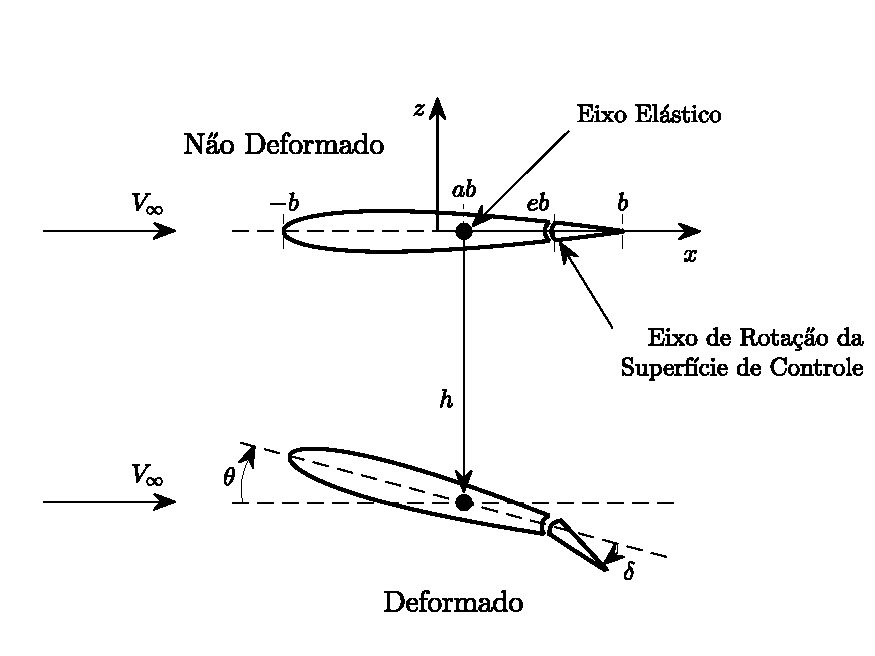
\includegraphics[width=\textwidth]{trabalho-graduacao/capitulos/figures/cap_2/secao-tipica.pdf}
    \label{fig:cap2:sistema-fisico}
\end{figure}

O referencial adotado contém a origem na posição de meia corda da seção, com os eixos conforme apresentados na figura. Os \gls{GDL}s que descrevem os movimentos de interesse são

\begin{itemize}
    \item Deslocamento linear vertical, \gls{h};
    \item Rotação da seção bidimensional em torno do eixo elástico, \gls{theta}.
\end{itemize}

Como já mencionado, o sistema é controlado por uma superfície de controle do tipo \textit{flap}, localizada no bordo de fuga da seção bidimensional podendo rotacionar em torno do eixo de rotação da superfície, localizado à uma distância $e$ em relação à origem, e representado pela variável $\gls{delta}$. Considerou-se que a dinâmica dessa superfície é determinada exclusivamente pela ação do atuador sobre a mesma, ou seja, negligenciaram-se os efeitos aeroelásticos associados ao seu movimento.

Além dos \gls{GDL}s e da superfície de controle, a Figura \ref{fig:cap2:sistema-fisico} apresenta os parâmetros físicos e geométricos que impactam na descrição do sistema. As indicações apresentadas na imagem se referem aos seguintes parâmetros:

\begin{itemize}
    \item \gls{Voo} representa a velocidade do escoamento não perturbado;
    \item \gls{b} é o valor da semi-corda da seção típica, a corda total é dada como \gls{c} $ = 2b$;
    \item \gls{a} é a posição relativa do eixo elástico a partir da posição de corda média, isto é, da origem do sistema de referência adotado;
    \item O eixo de rotação da superfície está a uma posição relativa igual a \gls{e} a partir da posição de corda média.
\end{itemize}


% ----------------------------------------------------------
\section{Equações do Movimento}\label{sec:equacoes-movimento}

Para o desenvolvimento das equações do movimento que descrevem o sistema aeroelástico, deve-se realizar o balanço dos esforços de inércia, aerodinâmicos, elásticos e os esforços externos que excitam o sistema \cite{book:Fung}. A forma geral para as equações que representam o sistema aeroelástico é definida segundo \textcite{book:Wright-Cooper}, como

\begin{equation} \label{eq:equacao-dinamica}
    \gls{M}\ddot{\gls{r}} +  \gls{D}\dot{\gls{r}} + \gls{K}\gls{r} = \boldsymbol{F}
\end{equation}

\noindent na qual as matrizes \gls{M} $\in \mathbb{R}^{\gls{NGDL} \times \gls{NGDL}}$, \gls{D} $\in \mathbb{R}^{\gls{NGDL} \times \gls{NGDL}}$ e \gls{K} $\in \mathbb{R}^{\gls{NGDL} \times \gls{NGDL}}$ são as matrizes de massa, amortecimento e rigidez do sistema, respectivamente. O vetor \gls{r} é o vetor de \gls{GDL}s, definido como,

\begin{equation} \label{eq:gdls}
    \gls{r} = \begin{bmatrix}
        \gls{h} & \gls{theta}
    \end{bmatrix}^{T}
\end{equation}

A dependência com o tempo de cada termo em \eqref{eq:equacao-dinamica} e \eqref{eq:gdls} foi omitida para claridade do texto. Em \eqref{eq:equacao-dinamica}, as parcelas $\gls{M}\ddot{\gls{r}}$, $\gls{D}\dot{\gls{r}}$ e $\gls{K}\gls{r}$ são, respectivamente as forças inerciais, de amortecimento e elástica referentes aos \gls{GDL}s do modelo estrutural, esses que são representados por \gls{r}. Mais ainda, \gls{F} representa as forças externas atuando sobre esses \gls{GDL}s. Neste trabalho serão consideradas as parcelas devido: aos esforços aerodinâmicos induzidos pela deformação estrutural, \gls{Fa}, à aerodinâmica imposta pela deflexão da superfície de controle, \gls{Fc} e ao esforço de reação inercial do movimento da superfície de controle, \gls{Fr}. Matematicamente, 

\begin{equation} \label{eq:forcas-aplicadas}
    \gls{F} = \gls{Fa} + \gls{Fc} + \gls{Fr}
\end{equation}

As parcelas de força provenientes de esforços aerodinâmicos devem ser calculadas contabilizando o efeito não estacionário do comportamento. Como discutido por \textcite{book:Wright-Cooper}, usualmente tais esforços são definidos no domínio da frequência utilizando-se da definição de frequência reduzida $k$, dada por

\begin{equation}\label{eq:Frequencia-reduzida}
    i\gls{k} = \frac{s\gls{b}}{\gls{Voo}}
\end{equation}

\noindent em que $s$ é a variável de Laplace, $i = \sqrt{-1}$ é a variável complexa e \gls{Voo} e \gls{b} representam a velocidade do escoamento não perturbado e o comprimento característico do modelo, respectivamente.

A força aerodinâmica devido à deformação estrutural pode ser dada por

\begin{equation} \label{eq:forca-aerodinamica}
    \gls{Fa} = \gls{qoo}\gls{AICa}(i\gls{k})\gls{r}
\end{equation}

\noindent sendo $\gls{qoo}=\frac{\gls{rho} \gls{Voo}}{2}$. O desenvolvimento matemático para obtenção de \eqref{eq:forca-aerodinamica} pode ser encontrado em \textcite{ZAERO-Theoretical-Manual:2017}. O termo $\gls{AICa} \in \mathbb{C}^{\gls{NGDL} \times \gls{NGDL}}$ em \eqref{eq:forca-aerodinamica} é a matriz de coeficientes de influência aerodinâmica, que é função da frequência reduzida e descreve o comportamento aerodinâmico não estacionário, como definida por \textcite{book:Wright-Cooper}. De maneira similar, a força aerodinâmica induzida pela deflexão da superfície de controle é dada por

\begin{equation} \label{eq:forca-superficie-controle}
    \gls{Fc} = \gls{qoo}\gls{AICc}(i\gls{k})\gls{delta}
\end{equation}

\noindent em que $\gls{delta}$ representa o ângulo de deflexão e $\gls{AICc} \in \mathbb{C}^{\gls{NGDL} \times 1}$ é a parcela da matriz de coeficientes de influência aerodinâmica referente à superfície de controle.

Estruturalmente, o movimento da superfície de controle induz uma força de reação na estrutura (aplicada nos \gls{GDL}s) definida por

\begin{equation} \label{eq:forca-reacao-superficie-controle}
    \gls{Fr} = -\gls{Mc}\ddot{\gls{delta}}
\end{equation}

\noindent sendo $\gls{Mc} \in \mathbb{R}^{\gls{NGDL} \times 1}$ a matriz de acoplamento inercial entre os \gls{GDL}s elásticos e da superfície de controle.

Assim, a equação \eqref{eq:equacao-dinamica} pode ser reescrita substituindo-se as forças definidas em \eqref{eq:forca-aerodinamica}, \eqref{eq:forca-superficie-controle} e \eqref{eq:forca-reacao-superficie-controle} resultando em

\begin{equation} \label{eq:equacao-dinamica2}
    \gls{M}\ddot{\gls{r}} +  \gls{D}\dot{\gls{r}} + \gls{D}\gls{r} = \gls{qoo}\gls{AICa}(i\gls{k})\gls{r} +  \gls{qoo}\gls{AICc}(i\gls{k})\gls{delta} - \gls{Mc}\ddot{\gls{delta}}
\end{equation}


Então, as equações do movimento de \eqref{eq:equacao-dinamica2} podem ser expressas de forma concisa no formato matricial como

\begin{equation} \label{eq:equacao-dinamica-final}
    \begin{bmatrix}
        \gls{M} & \gls{Mc}
    \end{bmatrix}
    \begin{bmatrix}
        \ddot{\gls{r}} \\ \ddot{\gls{delta}}
    \end{bmatrix}
    +
    \begin{bmatrix}
        \gls{D} & \boldsymbol{0}
    \end{bmatrix}
    \begin{bmatrix}
        \dot{\gls{r}} \\ \dot{\gls{delta}}
    \end{bmatrix}
    +
    \begin{bmatrix}
        \gls{K} & \boldsymbol{0}
    \end{bmatrix}
    \begin{bmatrix}
        \gls{r} \\ \gls{delta}
    \end{bmatrix}
    =
    \gls{qoo}\begin{bmatrix}
        \gls{AICa} & \gls{AICc}
    \end{bmatrix}
    \begin{bmatrix}
        \gls{r} \\ \gls{delta}
    \end{bmatrix}
\end{equation}

Para a seção bidimensional, as matrizes estruturais que definem o sistema, isto é $\gls{M}$, $\gls{D}$, $\gls{K}$ e $\gls{Mc}$, podem ser encontradas resolvendo as Equações de Lagrange para o sistema, conforme mostrado por \textcite{book:Wright-Cooper}, resultando em

\begin{equation}\label{eq:matriz-massa}
    \gls{M} = \begin{bmatrix}
        \gls{m} & S_{\theta} \\ S_{\theta} & I_{\theta} 
    \end{bmatrix}
\end{equation}

\begin{equation}\label{eq:matriz-amortecimento}
    \gls{D} = \begin{bmatrix}
        \xi_{h}(2m\omega_{h}) & 0 \\ 0 & \xi_{\theta}(2I_{\theta}\omega_{\theta}) 
    \end{bmatrix}
\end{equation}

\begin{equation}\label{eq:matriz-rigidez}
    \gls{K} = \begin{bmatrix}
        2m\omega^{2}_{h} & 0 \\ 0 & I_{\theta}\omega^{2}_{\theta} 
    \end{bmatrix}
\end{equation}

\begin{equation}\label{eq:matriz-acoplamento-inercial}
    \gls{Mc} = \begin{bmatrix}
        S_{\delta,h} \\ S_{\delta,\theta} 
    \end{bmatrix}
\end{equation}

\noindent sendo $\gls{csiGDL}$ e $\gls{omegaGDL}$, para $r_{k} = \{ \gls{h}, \ \gls{theta} \}$, respectivamente, amortecimentos e frequências naturais dos \gls{GDL}s desacoplados. Os parâmetros $S_{\theta}$ e $I_{\theta}$ representam o momento de massa estática e de inércia em relação ao eixo elástico, como definido por \textcite{book:Fung}. Além disso, $S_{\delta,h}$ e $S_{\delta,\theta}$ são os parâmetros de acoplamento inercial do movimento da superfície de controle aos \gls{GDL}s.

Vale comentar que, em \eqref{eq:equacao-dinamica-final}, omitiu-se a dependência da frequência reduzida das matrizes aerodinâmicas \gls{AICa} e \gls{AICc}. Porém, destaca-se que, apesar das equações do movimento serem apresentadas no domínio do tempo, os efeitos não-estacionários das matrizes aerodinâmicas devem ser expressos de forma a modelar no tempo os termos dependentes da frequência reduzida, o que será abordado na seção seguinte.

% ----------------------------------------------------------




% ----------------------------------------------------------
\section{Aproximação Aerodinâmica por Funções Racionais}\label{sec:rfa-solucao}

Apesar da descrição dos carregamentos em função de determinadas frequências reduzidas ser suficiente para caracterização das margens de estabilidade do sistema, essa abordagem prevê somente movimentos harmônicos e não possibilita a análise para movimentos arbitrários \cite{art:NASA1367}. Para analisar este último caso, que é o que ocorre quando o sistema contém \gls{AFS}, pode-se aproximar as matrizes aerodinâmicas dependentes da frequência reduzida por funções racionais, no domínio da frequência e, então, essa aproximação é transformada para o domínio do tempo. Essa técnica é conhecida como \gls{RFA}, e foi utilizada por em diversos trabalhos, como \textcite{book:Wright-Cooper, art:NASA1367, art:NASA2776, art:RogerRFA1977}.

Aplicando a transformada de Laplace em \eqref{eq:equacao-dinamica-final}, considerando condições iniciais nulas, é possível escrever

\begin{equation} \label{eq:equacao-dinamica-laplace}
    \begin{bmatrix}
         \left(\gls{M}s^2+\gls{D}s+\gls{K} \right) & \gls{Mc}
    \end{bmatrix}
    \begin{bmatrix}
        \gls{r}(s) \\ \gls{delta}(s)
    \end{bmatrix}
    =
    \gls{qoo}\begin{bmatrix}
        \gls{AICa} & \gls{AICc}
    \end{bmatrix}
    \begin{bmatrix}
        \gls{r}(s) \\ \gls{delta}(s)
    \end{bmatrix}
\end{equation}

Conforme descrito por \textcite{art:NASA1367}, o uso de \gls{RFA} consiste em aproximar as matrizes aerodinâmicas dependentes da frequência reduzida, $k$, por uma soma de termos racionais, como

\begin{multline}\label{eq:definicao-RFA}
    \boldsymbol{Q}_{aero}(ik) = 
    \begin{bmatrix}
        \gls{AICa}(ik) & \gls{AICc}(ik)
    \end{bmatrix}
    \approx \\
    \boldsymbol{A}_{0}^{RFA} + \boldsymbol{A}_{1}^{RFA}ik + \boldsymbol{A}_{2}^{RFA}(ik)^2 + \sum_{n=1}^{\gls{NL}} \frac{ik}{ik+\gls{pn}}\boldsymbol{A}_{n+2}^{RFA}
\end{multline}

\noindent em que,

\begin{equation}\label{eq:matrizes-RFA}
    \gls{Ai}^{RFA} = \begin{bmatrix}
        \boldsymbol{A}_{r,i}^{RFA} & \boldsymbol{A}_{c,i}^{RFA}
    \end{bmatrix} \in \mathbb{R}^{\gls{NGDL} \times \gls{NGDL}+1}, \quad i = 0, \ 1,\ 2,\ \cdots,\ \gls{NL}+2
\end{equation}

Na aproximação proposta em \eqref{eq:definicao-RFA} e \eqref{eq:matrizes-RFA}, $\gls{NL}$ e $\gls{pn}$ representam o número de termos de atraso e os polos desses termos, respectivamente. Esses parâmetros são variáveis de projeto a serem ajustadas no processo de aproximação e devem ser variados afim de encontrar o conjunto que melhor aproxima as matrizes \gls{RFA} das $\boldsymbol{AIC}$s \cite{book:Wright-Cooper}.

Para valores estipulados dos parâmetros de atraso, o processo de solução de \eqref{eq:definicao-RFA} proposto por \textcite{art:RogerRFA1977} consiste em encontrar as matrizes $\boldsymbol{A}_{0},\  \boldsymbol{A}_{1},\  ...,\  \boldsymbol{A}_{n+2}$ minimizando o erro da aproximação em relação às matrizes aerodinâmicas. Em particular, utiliza-se para avaliação o erro quadrático para cada elemento $ij$ das matrizes como

\begin{multline}\label{eq:erro-aproximacao-RFA}
    \varepsilon_{ij} = \sum_{m=1}^{\gls{Nk}} \left( \boldsymbol{A}_{0} + \boldsymbol{A}_{1}ik_{m} + \boldsymbol{A}_{2}(ik_{m})^2 + \sum_{n=1}^{\gls{NL}} \frac{\boldsymbol{A}_{n+2}}{ik_{m}+\gls{pn}}ik_{m} - \boldsymbol{Q}_{aero}(k_{m}) \right)_{ij} ^2 , \\ i = 1,\ 2,\ \cdots,\ \gls{NGDL} \ \text{e}, \ j = 1,\ 2,\ \cdots,\ \gls{NGDL}+1
\end{multline}

\noindent sendo $\gls{Nk}$ o número de frequências reduzidas utilizadas na determinação das matrizes $\boldsymbol{AIC}$.

O objetivo da aproximação é minimizar o erro entre a soma de funções racionais e as matrizes aerodinâmicas $\boldsymbol{AIC}$ para cada frequência reduzida $k$ na qual foram determinadas. Isto é, deseja-se que $\varepsilon_{ij} = 0$. Logo, como descrito por \textcite{book:Wright-Cooper}, é possível escrever a solução para os termos das matrizes de aproximação a partir de \eqref{eq:erro-aproximacao-RFA} como

\begin{equation}\label{eq:solucao-RFA}
    \begin{bmatrix}
    1 & ik_{1} & -k_{1} & \frac{ik_{1}}{ik_{1}+p_{1}} & \cdots & \frac{ik_{1}}{ik_{1}+p_{N_{L}}} \\
    1 & ik_{2} & -k_{2} & \frac{ik_{2}}{ik_{2}+p_{1}} & \cdots & \frac{ik_{2}}{ik_{2}+p_{N_{L}}} \\
    \vdots & \vdots & \vdots & \vdots & & \vdots \\
    1 & ik_{N_{k}} & -k_{N_{k}} & \frac{ik_{N_{k}}}{ik_{N_{k}}+p_{1}} & \cdots & \frac{ik_{N_{k}}}{ (ik_{N_{k}}+p_{N_{L}}) } \\
    \end{bmatrix} 
    \begin{bmatrix}
    \boldsymbol{A}_{0} \\ \boldsymbol{A}_{1} \\ \boldsymbol{A}_{2} \\ \vdots \\ \boldsymbol{A}_{N_{L}+2}
    \end{bmatrix} _{ij}
    = 
    \begin{bmatrix}
    \boldsymbol{Q}_{aero}(ik_{1}) \\ \boldsymbol{Q}_{aero}(ik_{2}) \\ \vdots \\ \vdots \\ \boldsymbol{Q}_{aero}(ik_{N_{k}})
    \end{bmatrix} _{ij}
\end{equation}

Resolvendo \eqref{eq:solucao-RFA} para cada elemento $ij$ das matrizes de aproximação, tem-se a \gls{RFA} completa para os parâmetros de atraso determinados. A aproximação deve ser avaliada, para todos os pontos de frequência reduzida que descrevem a aerodinâmica não-estacionária do modelo. Como discutido por \textcite{ZAERO-Theoretical-Manual:2017}, o aumento do número de termos utilizados, isto é, maiores valores de $N_{L}$, reduzirá o erro da aproximação. Porém, esse aumento resulta no aumento de variáveis de estado do modelo, aumentando o custo computacional para as soluções.

Uma vez obtidas as matrizes aerodinâmicas de aproximação pode-se reescrever \eqref{eq:equacao-dinamica-laplace} como

\begin{multline}\label{eq:equacao-dinamica-laplace-RFA}
    \begin{bmatrix}
         \left(\gls{M}s^2+\gls{D}s+\gls{K} \right) & \gls{Mc}
    \end{bmatrix}
    \begin{bmatrix}
        \gls{r}(s) \\ \gls{delta}(s)
    \end{bmatrix} \\
    =
    \gls{qoo} \left( 
    \boldsymbol{A}_{0} + \boldsymbol{A}_{1}ik + \boldsymbol{A}_{2}(ik)^2 + \sum_{n=1}^{\gls{NL}} \frac{ik}{ik+\gls{pn}}\boldsymbol{A}_{n+2} \right)
    \begin{bmatrix}
        \gls{r}(s) \\ \gls{delta}(s)
    \end{bmatrix}
\end{multline}

Utilizando \eqref{eq:Frequencia-reduzida}, \eqref{eq:matrizes-RFA} e aplicando a transformada inversa de Laplace em \eqref{eq:equacao-dinamica-laplace-RFA}, segue que

\begin{multline}\label{eq:equacao-movimento-RFA}
    \left(\gls{M} - \gls{qoo}\frac{b^2}{\gls{Voo}^2}\boldsymbol{A}_{r,2}\right)\ddot{\gls{r}} + \left(\gls{D} - \gls{qoo}\frac{b}{\gls{Voo}}\boldsymbol{A}_{r,1} \right) \dot{\gls{r}} +  \left(\gls{K} - \gls{qoo}\boldsymbol{A}_{r,0} \right)\gls{r} \\ - \gls{qoo}\sum_{n=1}^{N_{L}}\boldsymbol{X}_{A,n} + \left(\gls{Mc} - \gls{qoo}\frac{b^2}{\gls{Voo}^2}\boldsymbol{A}_{c,2}\right)\ddot{\gls{delta}} - \gls{qoo}\frac{b}{\gls{Voo}}\boldsymbol{A}_{c,1} \dot{\gls{delta}} - \gls{qoo}\boldsymbol{A}_{c,0}\gls{delta} = 0
\end{multline}

\noindent em que $\gls{Xa} \in \mathbb{R}^{ \gls{NGDL} \times 1}$ representam os estados aumentados devido ao atraso aerodinâmico, e são definidos como proposto por \textcite{art:NASA2776} a partir dos temos $n+2$, sendo $\ n=1,\ 2,\ \cdots, \ \gls{NL}$, da aproximação, como

\begin{equation}\label{eq:estados-atraso-aerodinamicos}
    \boldsymbol{X}_{A,n}(s) = \boldsymbol{A}_{n+2}\frac{ik}{ik+\gls{pn}}
    \begin{bmatrix}
        \gls{r}(s) \\ \gls{delta}(s)
    \end{bmatrix}, \ n = 1,\ 2,\ \cdots,\ \gls{NL} 
\end{equation}

Utilizando a definição da frequência reduzida dada em \eqref{eq:Frequencia-reduzida}, é possível reescrever \eqref{eq:estados-atraso-aerodinamicos} em função da variável de Laplace, obtendo

\begin{equation}\label{eq:estados-atraso-aerodinamicos-laplace}
    \boldsymbol{X}_{A,n}(s) = \boldsymbol{A}_{n+2}\frac{1}{s+\frac{\gls{Voo}}{\gls{b}}\gls{pn}}
    s\begin{bmatrix}
        \gls{r}(s) \\ \gls{delta}(s)
    \end{bmatrix}, \ n = 1,\ 2,\ \cdots,\ \gls{NL} 
\end{equation}

No domínio do tempo, os estados de atraso podem ser encontrados pela integral de convolução entre as transformadas inversas de Laplace dos dois termos de \eqref{eq:estados-atraso-aerodinamicos-laplace}, evidenciando a relação entre os estados associados ao movimento e os associados ao atraso aerodinâmico. Matematicamente, tem-se

\begin{equation}\label{eq:estados-atraso-aerodinamicos-tempo}
    \boldsymbol{X}_{A,n}(t) = \int_{0}^{t} \boldsymbol{A}_{n+2}e^{-\left(\frac{\gls{Voo}}{\gls{b}}\right)\gls{pn}(t-\tau)} \begin{bmatrix}
        \dot{\gls{r}} \\ \dot{\gls{delta}}
    \end{bmatrix}  d\tau, \ n = 1,\ 2,\ \cdots,\ \gls{NL} 
\end{equation}

Derivando \eqref{eq:estados-atraso-aerodinamicos-tempo} pode-se encontrar a equação dinâmica que descreve o comportamento dos termos de atraso aerodinâmico, dada por 

\begin{align}\label{eq:estados-atraso-aerodinamicos-derivada}
\begin{split}
    \boldsymbol{\dot{X}}_{A,n}(t) & = \boldsymbol{A}_{n+2} \begin{bmatrix}
        \dot{\gls{r}} \\ \dot{\gls{delta}}
    \end{bmatrix} - \left(\frac{\gls{Voo}}{\gls{b}}\right)\gls{pn}\boldsymbol{X}_{A,n}(t) \\
    & = \boldsymbol{A}_{r,n+2}\dot{\gls{r}} + \boldsymbol{A}_{c,n+2}\dot{\gls{delta}} - \left(\frac{\gls{Voo}}{\gls{b}}\right)\gls{pn}\boldsymbol{X}_{A,n}(t), \ n = 1,\ 2,\ \cdots,\ \gls{NL} 
\end{split}
\end{align}

A utilização da técnica de aproximação por funções racionais apresenta a possibilidade de aproximar carregamentos provenientes de diferentes métodos de análises aerodinâmicas, como, por exemplo, resultados de análise de fluidodinâmica computacional, experimentos em túnel de vento ou ensaios em voo \cite{book:Wright-Cooper}.

A principal desvantagem dessa metodologia é a introdução de diversos novos estados no modelo dinâmico. Neste trabalho, considerar-se-ão quatro termos de atraso. Logo, o modelo resultante terá $15$ estados, como será abordado a seguir.

% ----------------------------------------------------------

% ----------------------------------------------------------
\section{Representação no Espaço de Estados}\label{sec:espaço-estados}

Com o objetivo de avaliar comportamento dinâmico em malha aberta e em fechada do modelo desenvolvido, as equações dinâmicas que descrevem o sistema são representadas no espaço de estados, isto é, na forma

\begin{equation}\label{eq:espaco-estados-completo}
    \begin{gathered}
        \dot{\boldsymbol{x}} = \boldsymbol{A}\boldsymbol{x} + \boldsymbol{B}u_{c} \\
        \boldsymbol{y} = \boldsymbol{C}\boldsymbol{x}
    \end{gathered}
\end{equation}

\noindent em que $\gls{x} \in \mathbb{R}^{N_x}$ é o vetor de estados, variáveis internas da planta que determinam a dinâmica do sistema, $\gls{uc}$ é a entrada, parâmetros controláveis da planta, no caso, a deflexão comandada da superfície de controle, $\gls{y} \in \mathbb{R}^{N_y}$ é o vetor de saída, variáveis de interesse do sistema, $\gls{A} \in \mathbb{R}^{\gls{Nx} \times \gls{Nx}}$ é a matriz dinâmica e representa a dinâmica do sistema sendo modelado, $\gls{B} \in \mathbb{R}^{\gls{Nx} \times 1}$ é a matriz de entrada que relaciona a entrada do sistema à dinâmica da planta, e $\gls{C} \in \mathbb{R}^{\gls{Ny} \times \gls{Nx}}$ é a matriz de saída e relaciona as variáveis de estado do sistema à saída de interesse.

No presente trabalho, o vetor de estados é composto por deslocamentos e velocidades dos \gls{GDL}s, os vetores de estados de atraso, $\boldsymbol{X}_{A,n}, \ n = 1,\ 2,\ \cdots,\ \gls{NL}$, provenientes da aproximação por \gls{RFA}, e os estados internos do atuador, que representam a deflexão da superfície de controle e sua velocidade e aceleração. Matematicamente,

\begin{equation}\label{eq:definicao-estados-geral}
    \boldsymbol{x} = \begin{bmatrix} \gls{r}^{T} & \dot{\gls{r}}^{T} & \boldsymbol{X}_{A,1}^{T} & \cdots & \boldsymbol{X}_{A,N_L}^{T} & \gls{delta} & \dot{\gls{delta}} & \ddot{\gls{delta}} \end{bmatrix}^{T}
\end{equation}

Com exceção dos três últimos estados, os elementos que compõem o vetor definido em \eqref{eq:definicao-estados-geral} têm dimensão igual ao número de \gls{GDL}s. Assim, percebe-se que o número de estados depende tanto do número de \gls{GDL}s do sistema quanto da quantidade de termos de atraso utilizados para a aproximação dos carregamentos aerodinâmicos e dos estados da dinâmica do atuador. Matematicamente, a dimensão do vetor de estados é dada por

\begin{equation}\label{Eq_NoEstados}
    \gls{Nx} = \left( 2  + \gls{NL} \right)\gls{NGDL} + 3
\end{equation}

No presente trabalho, têm-se dois graus de liberdade como definido em \eqref{eq:gdls}, isto é, \gls{NGDL} $=2$, representando o deslocamento vertical e a rotação da seção bidimensional.

O modelo aeroservoelástico definido em \eqref{eq:espaco-estados-completo} é composto pelo modelo aeroelástico representado por \eqref{eq:equacao-movimento-RFA} e \eqref{eq:estados-atraso-aerodinamicos-derivada} e pela dinâmica do atuador. Assim, para determinação das matrizes que compõem \eqref{eq:espaco-estados-completo}, será descrita a modelagem no espaço de estados dessas três dinâmicas (aeroelástica, atraso aerodinâmico e atuador). Por fim, será realizada a integração dos modelos na representação no espaço de estados final.

Para o modelo aeroelástico, pode simplificar a representação de \eqref{eq:equacao-movimento-RFA} definindo as matrizes $\boldsymbol{\Tilde{M}}$, $\boldsymbol{\Tilde{D}}$, $\boldsymbol{\Tilde{K}}$ e $\boldsymbol{\Tilde{M}}_{c}$ como

\begin{equation}\label{Eq_MatrizesSimplificacao1}
    \boldsymbol{\Tilde{M}} = \left(\gls{M} - \gls{qoo}\frac{b^2}{\gls{Voo}^2}\boldsymbol{A}_{r,2}\right)
\end{equation}
\begin{equation}\label{Eq_MatrizesSimplificacao2}
    \boldsymbol{\Tilde{D}} = \left(\gls{D} - \gls{qoo}\frac{b}{\gls{Voo}}\boldsymbol{A}_{r,1}\right)
\end{equation}
\begin{equation}\label{Eq_MatrizesSimplificacao3}
    \boldsymbol{\Tilde{K}} = \left(\gls{K} - \gls{qoo}\boldsymbol{A}_{r,0}\right)
\end{equation}
\begin{equation}\label{Eq_MatrizesSimplificacao4}
    \boldsymbol{\Tilde{M}}_{c} = \left(\boldsymbol{M}_{c} - \gls{qoo}\frac{b^2}{\gls{Voo}^2}\boldsymbol{A}_{c,2}\right)
\end{equation}

Então, rearranjando \eqref{eq:equacao-movimento-RFA}, é possível escrever

\begin{multline}\label{eq:equacao-movimento-RFA-simplificada}
   \ddot{\gls{r}} =  -\boldsymbol{\Tilde{M}}^{-1}\boldsymbol{\Tilde{D}}\dot{\gls{r}} -\boldsymbol{\Tilde{M}}^{-1}\boldsymbol{\Tilde{K}}\gls{r} +\boldsymbol{\Tilde{M}}^{-1}\gls{qoo}\sum_{n=1}^{N_{L}}\boldsymbol{X}_{A,n} \\ -\boldsymbol{\Tilde{M}}^{-1}\boldsymbol{\Tilde{M}}_{c}\ddot{\gls{delta}} +\gls{qoo}\frac{b}{\gls{Voo}}\boldsymbol{\Tilde{M}}^{-1}\boldsymbol{A}_{c,1} \dot{\gls{delta}} + \gls{qoo}\boldsymbol{\Tilde{M}}^{-1}\boldsymbol{A}_{c,0}\gls{delta}
\end{multline}

Assim, a representação no espaço de estados para o modelo aeroelástico pode ser definida a partir de \eqref{eq:equacao-movimento-RFA-simplificada} e \eqref{eq:estados-atraso-aerodinamicos-derivada} como

\begin{equation}\label{eq:espaço-estados-aeroelastico}
    \dot{\boldsymbol{x}}_{ae} = \boldsymbol{A}_{ae}\boldsymbol{x}_{ae} + \boldsymbol{B}_{ae}\boldsymbol{u}_{ae}
\end{equation}

\noindent em que os vetores de estados $\gls{xae}$ e entrada $\gls{uae}$ são definidos por

\begin{equation}\label{eq:ss-aeroelastico-definicao}
\begin{gathered}
    \gls{xae} = \begin{bmatrix}
        \gls{r} \\ \boldsymbol{\dot{\gls{r}}} \\ \boldsymbol{X}_{A,1} \\ \vdots \\ \boldsymbol{X}_{A,N_{L}}
    \end{bmatrix}, 
    \ \text{e} \ 
    \gls{uae} = \begin{bmatrix}
        \gls{delta} \\ \dot{\gls{delta}} \\ \ddot{\gls{delta}}
    \end{bmatrix}
\end{gathered}
\end{equation}

\noindent e as matrizes que compõe a representação são

\begin{equation}\label{eq:matriz-dinamica-aeroelastico}
    \gls{Aae} = \begin{bmatrix}
    \boldsymbol{0}                                               & \boldsymbol{I}                                               & \boldsymbol{0}                                 & \boldsymbol{0} & \cdots & \boldsymbol{0} \\
    -\boldsymbol{\Tilde{M}}^{-1}\boldsymbol{\Tilde{K}} & -\boldsymbol{\Tilde{M}}^{-1}\boldsymbol{\Tilde{D}} &  \gls{qoo}\boldsymbol{\Tilde{M}}^{-1}    &  \gls{qoo}\boldsymbol{\Tilde{M}}^{-1}  & \cdots & \gls{qoo}\boldsymbol{\Tilde{M}}^{-1} \\
    \boldsymbol{0}                                               & \boldsymbol{A}_{r,3}                                         & -\left( \frac{V}{b} \right)p_{1}\boldsymbol{I} & \boldsymbol{0} & \cdots & \boldsymbol{0} \\
    \boldsymbol{0}                                               & \boldsymbol{A}_{r,4}                                 & \boldsymbol{0}                                 & -\left( \frac{V}{b} \right)p_{2}\boldsymbol{I} & \cdots & \boldsymbol{0} \\
    \vdots & \vdots & \vdots & \vdots & \ddots & \vdots \\
    \boldsymbol{0}                                               & \boldsymbol{A}_{r,N_{L}+2}                                 & \boldsymbol{0}                                 & \cdots & \boldsymbol{0}  & -\left( \frac{V}{b} \right)p_{N_{L}}\boldsymbol{I}  \\
    \end{bmatrix}
\end{equation}

\begin{equation}\label{eq:matriz-controle-aeroelastico}
    \gls{Bae} = \begin{bmatrix}
        \boldsymbol{0} & \boldsymbol{0} & \boldsymbol{0} \\
        -\boldsymbol{\Tilde{M}}^{-1}\boldsymbol{\Tilde{M}}_{c} & \gls{qoo}\frac{b}{\gls{Voo}}\boldsymbol{\Tilde{M}}^{-1}\boldsymbol{A}_{c,1} & \gls{qoo}\boldsymbol{\Tilde{M}}^{-1}\boldsymbol{A}_{c,0} \\
        \boldsymbol{0} & \boldsymbol{A}_{c,3} & \boldsymbol{0} \\
        \vdots & \vdots & \vdots \\
        \boldsymbol{0} & \boldsymbol{A}_{c,N_{L}+2} & \boldsymbol{0}
    \end{bmatrix}
\end{equation}

Como discutido em \textcite{art:Huang-2015}, a superfície de controle não apresenta uma resposta instantânea aos comandos do controlador, dado a inércia do movimento da superfície. Para a determinação do modelo que representa a dinâmica do sistema aeroelástico como um todo, faz-se necessário representar a dinâmica do atuador que controla o movimento da superfície de controle utilizada. Para isso, utilizou-se uma função de transferência de terceira ordem proposta por \textcite{art:Huang-2015, ZAERO-Theoretical-Manual:2017}. Especificamente, considerou-se que a dinâmica entre o ângulo comandado $u_{c}$ e o ângulo real de deflexão $\gls{delta}$ da superfície de controle é descrita, no espaço de estados, por

\begin{equation}\label{eq:modelo-atuador}
    \dot{\boldsymbol{\gls{delta}}} = \gls{Aac}\boldsymbol{\gls{delta}} + \gls{Bac}\gls{uc}
\end{equation}

\noindent em que

\begin{equation}\label{eq:matrizes-modelo-atuador}
    \boldsymbol{\gls{delta}} = \begin{bmatrix}
        \gls{delta} \\ \dot{\gls{delta}} \\ \ddot{\gls{delta}}
    \end{bmatrix}; \quad
    \gls{Aac} = 
    \begin{bmatrix}
    0 & 1 & 0 \\
    0 & 0 & 0 \\
    -Z_{0}\omega_{ac}^{3} & -Z_{1}\omega_{ac}^{2} & -Z_{2}\omega_{ac}
    \end{bmatrix}; \quad
    \gls{Bac} = 
    \begin{bmatrix}
    0 \\ 0 \\ Z_{0}\omega_{ac}^{3}
    \end{bmatrix};
\end{equation}

\noindent e $Z_{0}$, $Z_{1}$, $Z_{2}$ e $\omega_{ac}$ são parâmetros do atuador.

Finalmente, o modelo aeroservoelástico completo no espaço de estados definido em \eqref{eq:espaco-estados-completo} é encontrado manipulando \eqref{eq:espaço-estados-aeroelastico} e \eqref{eq:modelo-atuador}, resultando nas seguintes matrizes:

\begin{equation}\label{eq:matrizes-modelo-completo}
    \gls{A} = \begin{bmatrix}
        \gls{Aae} & \gls{Bae} \\
        \boldsymbol{0}      & \gls{Aac}
    \end{bmatrix}, \  
    \gls{B} = \begin{bmatrix}
        \boldsymbol{0} \\ \gls{Bac}
    \end{bmatrix}, \ 
    \gls{C} = \boldsymbol{I}_{N_{x}}
\end{equation}

Vale notar que, no desenvolvimento da lei de controle realizado no Capítulo \ref{cap:descricao-controle}, supõe-se que todos os estados são medidos. Por isso, em \eqref{eq:matrizes-modelo-completo} a matriz de saída é uma identidade.

% ----------------------------------------------------------
